\documentclass{beamer}

\usepackage{ctex}
\usepackage{subfigure}
\usepackage{CJK}
\usepackage{siunitx}
\usepackage{amsmath}
\usepackage{amssymb}
\usepackage{graphicx}
\usepackage{cite}
\usepackage{multirow}
\usepackage{float}
\usepackage{xltxtra}

\usetheme{Berlin}
\usecolortheme{seahorse}
%\usefonttheme

\begin{document}

\title{Julia Set 的生成}

\author{唐浩 \\ 信息与计算科学 3200102118}

\institute{浙江大学数学科学学院}
%\begin{document}

\maketitle

\begin{frame}
  \frametitle{正文}
  \begin{itemize}
  \item 引言
  \item 数学理论
  \item 算法
  \item 数值算例
  \item 分析
  \item 结论
  \end{itemize}
\end{frame}


\begin{frame}
  \frametitle{引言}
  \begin{columns}
    \column{0.3\textwidth}
    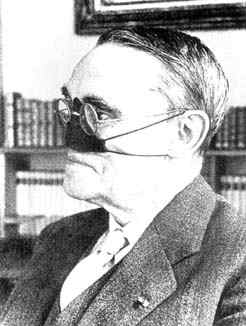
\includegraphics[scale=0.2]{Julia.jpeg}

    \column{0.7\textwidth}
  朱利亚集合(Julia Set)是一个在复平面上形成分形的点的集合。以法国数学家Gaston Julia的名字命名。
  
  它是一个几何图形,其中的点均出自迭代公式:{\bf $Z_{n+1} = Z_n^2 + C$},取定一个常数C, 对于复平面上的每一点 z,若$Z_n$收敛,则 z 在集合中。对于所有的 z 组成的集合,便称为{\bf Julia Set}。本文主要介绍如何生成 Julia Set,并简单叙述其与 Mandelbrot Set 之间的关系。
  \end{columns}
\end{frame}

\begin{frame}
  \frametitle{数学理论}
  \begin{columns}
    \column{0.4\textwidth}
    \begin{itemize}
    \item 迭代
    \end{itemize}
    迭代是重复反馈过程的活动。每一次对过程的重复称为一次“迭代”,而每一次迭代得到的结果会作为下一次迭代的初始值。就 Julia Set 而言,被迭代的是一些最简单的函数,其形如 $f(x) = x^2 + C$(C 为常量)。
    \column{0.6\textwidth}
    \begin{itemize}
    \item 逃逸时间算法
    \end{itemize}
    如果对于一个复数序列 $\{z_1, z_2, \dots, z_n\}$ 有 $|z_j| > max(2,|C|)$ 则序列将逃逸到无穷大。

    对于每个复参数平面上的点C,我们生成一个序列Z,根据逃逸准则,我们规定R为逃逸半径,在 $\{z_1, \dots z_n\}$ 里,如果 $|z_j| < R$ ,判断有界(但其实也有可能这个序列是无界的),反之,这个序列无界。
  \end{columns}
\end{frame}

\begin{frame}
  \frametitle{算法}
  \begin{figure}
    \centering
    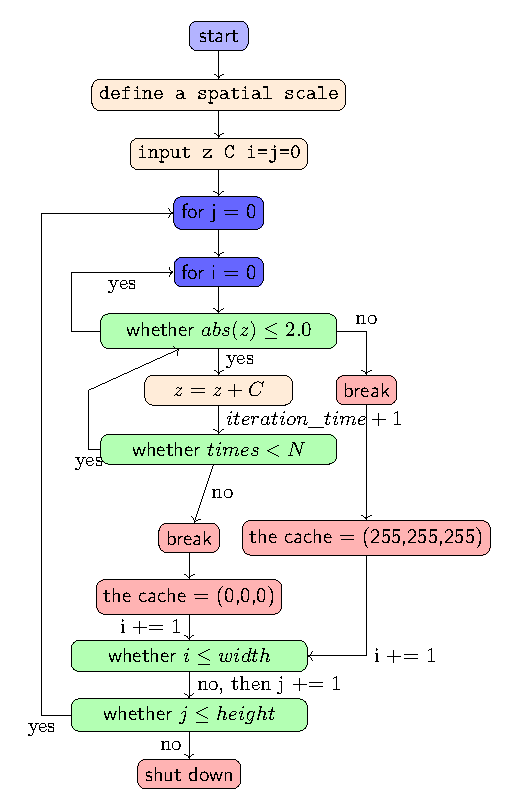
\includegraphics[scale=0.5]{julia.pdf}
  \end{figure}
\end{frame}

\begin{frame}
  \frametitle{数值算例}
  选取迭代次数 N = 100,选取不同的常数 C, 将会得到不同的 Julia Set,以下我们选取几个常数 C 的值,当我们将 C 设置成(0,0),将会得到一个圆,由于图像的对称性,在此,统一将 C 取为(-x,y)的形式。
  \begin{figure}[H]
    \centering
    \subfigure[C = (0,0)]
              {
                \centering
                \includegraphics[width=0.24\textwidth]{test0.bmp}
              }
    \subfigure[C = (-0.5,0.5)]
              {
                 \centering
                 \includegraphics[width=0.24\textwidth]{test7.bmp}
              }
  \end{figure}
  \begin{figure}[H]
    \centering
    \subfigure[C = (-0.1,0.7)]
              {
                \centering
                \includegraphics[width=0.24\textwidth]{test8.bmp}
              }
    \subfigure[C = (-1,0.2)]
              {
                 \centering
                 \includegraphics[width=0.24\textwidth]{test9.bmp}
              }
  \end{figure}
\end{frame}

\begin{frame}
  \frametitle{分析}
  \begin{figure}[H]
  \includegraphics[width=0.4\textwidth]{test3.bmp}
  \caption{This is a Mandelbrot Set picture}
  \end{figure}
  图中的每个点对应于一个filled Julia Set,其中黑点是路径连通的 Julia Set,白点是不连通的 Julia Set。选取 Mandelbrot Set 中的对应黑点,便可得到上面生成的 Julia Set 图。

  Mandelbrot Set 与 Julia Set 都是由迭代关系: $z_{n+1} = z_n + C$ 所产生的点集,只不过两者一个由 z 产生,一个由 C 产生,在计算机上表现的不同便是一个遍历 z ,一个遍历 C 
\end{frame}

\begin{frame}
  \frametitle{结论}
  Mandelbrot Set 与 Julia Set 都是由迭代关系: $z_{n+1} = z_n + C$ 所产生的点集,只不过两者一个由 z 产生,一个由 C 产生,在计算机上表现的不同便是一个遍历 z ,一个遍历C。
\end{frame}

\end{document}
